\documentclass{beamer}
\usepackage[utf8]{inputenc}

\usetheme{Madrid}
\usecolortheme{default}
\usepackage{amsmath,amssymb,amsfonts,amsthm}
\usepackage{txfonts}
\usepackage{tkz-euclide}
\usepackage{listings}
\usepackage{adjustbox}
\usepackage{array}
\usepackage{tabularx}
\usepackage{gvv}
\usepackage{lmodern}
\usepackage{circuitikz}
\usepackage{tikz}
\usepackage{graphicx}
\usepackage{multicol}
\setbeamertemplate{page number in head/foot}[totalframenumber]

\usepackage{tcolorbox}
\tcbuselibrary{minted,breakable,xparse,skins}



\definecolor{bg}{gray}{0.95}
\DeclareTCBListing{mintedbox}{O{}m!O{}}{%
  breakable=true,
  listing engine=minted,
  listing only,
  minted language=#2,
  minted style=default,
  minted options={%
    linenos,
    gobble=0,
    breaklines=true,
    breakafter=,,
    fontsize=\small,
    numbersep=8pt,
    #1},
  boxsep=0pt,
  left skip=0pt,
  right skip=0pt,
  left=25pt,
  right=0pt,
  top=3pt,
  bottom=3pt,
  arc=5pt,
  leftrule=0pt,
  rightrule=0pt,
  bottomrule=2pt,

  colback=bg,
  colframe=orange!70,
  enhanced,
  overlay={%
    \begin{tcbclipinterior}
    \fill[orange!20!white] (frame.south west) rectangle ([xshift=20pt]frame.north west);
    \end{tcbclipinterior}},
  #3,
}
\lstset{
    language=C,
    basicstyle=\ttfamily\small,
    keywordstyle=\color{blue},
    stringstyle=\color{orange},
    commentstyle=\color{green!60!black},
    numbers=left,
    numberstyle=\tiny\color{gray},
    breaklines=true,
    showstringspaces=false,
}
%------------------------------------------------------------
%This block of code defines the information to appear in the
%Title page
\title %optional
{1.1.12}
%\subtitle{A short story}

\author % (optional)
{BEERAM MADHURI - EE25BTECH11012}



\begin{document}


\frame{\titlepage}
\begin{frame}{Question}
Given closed-loop transfer function $T(s) = \frac{s-5}{(s+2)(s+3)}$, the system is: \hfill (EC 2007)

\begin{enumerate}
    \item[a)] Unstable
    \item[b)] Uncontrollable
    \item[c)] Minimum phase
    \item[d)] Non-minimum phase
\end{enumerate}
\end{frame}

\begin{frame}{solution}
    \frametitle{finding the Property of given system}
Given the closed-loop transfer function:
\begin{align}
    T(s) = \frac{s - 5}{(s + 2)(s + 3)}
\end{align}
Identifiying Poles and Zeros\\
\textbf{Poles:}\\
Set the denominator to zero: \\
\begin{align}
    (s + 2)(s + 3) = 0\\
    s = -2 ,-3
\end{align}
 Both are in the Left Half Plane (LHP).
\end{frame}
\begin{frame}
    \textbf{Zeros:}\\
Set the numerator to zero: 
\begin{align}{}
    s - 5 = 0\\
    s = +5
\end{align}
This is in the Right Half Plane (RHP).\\

Determining the System Property:\\
Since we have a zero at $s = 5$, the system is non-minimum phase.\\
Correct Option: d) Non-minimum phase
\end{frame}
\begin{frame}{}
    Given Options:\\
a) Unstable:\\
A system is unstable if any of its poles lie in the Right Half Plane (RHP) or if there are repeated poles on the imaginary axis.\\
Examples:\\
Stable: A commercial plane naturally stays level. If hit by wind, it corrects itself.\\
Unstable: A fighter jet without its computer would flip over and crash immediately.\\

\end{frame}

\begin{frame}{}
b)Uncontrollable:\\
A property related to State-Space analysis. In transfer functions, it usually implies a pole-zero cancellation. Since no terms cancel out here, we cannot assume it is uncontrollable from this form.\\

Examples:\\
Controllable: Every joint in a robotic arm moves when we tell it to. we can reach any point in space.\\

Uncontrollable: If a motor breaks, certain positions become impossible to reach, no matter what buttons we press.\\
\end{frame}

\begin{frame}
c)Minimum Phase:\\
A system where all poles and all zeros lie in the Left Half Plane (LHP). These systems have the minimum possible phase shift for a given magnitude response.\\

Examples:\\
Minimum Phase: You turn a car steering wheel right, and the car moves right immediately.\\
\end{frame}
\begin{frame}
d)Non-minimum Phase:\\
A system that has at least one zero (or pole) in the Right Half Plane (RHP). These systems exhibit "undershoot" in their step response and have more phase lag than a minimum phase system.\\

Examples:\\
Non-Minimum Phase: Like a large ship or forklift. To turn right, the back must swing left first. It moves the wrong way before going the right way.
\end{frame}

\begin{frame}[fragile]
\frametitle{C Code}
\begin{lstlisting}
#include <stdio.h>
#include <complex.h>
#include <math.h>

#define MAX_DEGREE 10
#define ITERATIONS 1000

// Function to evaluate polynomial at a complex point x
double complex evaluate(double coeff[], int degree, double complex x) {
    double complex res = coeff[degree];
    for (int i = degree - 1; i >= 0; i--) {
        res = res * x + coeff[i];
    }
    return res;
}
\end{lstlisting}
\end{frame}

\begin{frame}[fragile]
\frametitle{C Code}
\begin{lstlisting}
// Root finding using Durand-Kerner algorithm
void find_roots(double coeff[], int degree, double complex roots[]) {
    if (degree == 0) return;
    
    // Initial guesses for roots (complex numbers on a circle)
    for (int i = 0; i < degree; i++) {
        roots[i] = cpow(0.4 + 0.9 * I, i);
    }
\end{lstlisting}
\end{frame}

\begin{frame}[fragile]
\frametitle{C Code}
\begin{lstlisting}
    for (int iter = 0; iter < ITERATIONS; iter++) {
        for (int i = 0; i < degree; i++) {
            double complex denom = 1.0;
            for (int j = 0; j < degree; j++) {
                if (i != j) denom *= (roots[i] - roots[j]);
            }
            roots[i] -= evaluate(coeff, degree, roots[i]) / (coeff[degree] * denom);
        }
    }
}
\end{lstlisting}
\end{frame}

\begin{frame}[fragile]
\frametitle{C Code}
\begin{lstlisting}
int main() {
    int n_deg, d_deg;
    double num[MAX_DEGREE], den[MAX_DEGREE];
    double complex zeros[MAX_DEGREE], poles[MAX_DEGREE];

    printf("Enter degree of Numerator: ");
    scanf("%d", &n_deg);
    printf("Enter coefficients (from constant to highest power):\n");
    for(int i = 0; i <= n_deg; i++) scanf("%le", &num[i]);
\end{lstlisting}
\end{frame}

\begin{frame}[fragile]
\frametitle{C Code}
\begin{lstlisting}
    printf("\nEnter degree of Denominator: ");
    scanf("%d", &d_deg);
    printf("Enter coefficients (from constant to highest power):\n");
    for(int i = 0; i <= d_deg; i++) scanf("%le", &den[i]);

    find_roots(num, n_deg, zeros);
    find_roots(den, d_deg, poles);
\end{lstlisting}
\end{frame}

\begin{frame}[fragile]
\frametitle{C Code}
\begin{lstlisting}
    printf("TYPE,REAL,IMAG\n");
    for(int i = 0; i < n_deg; i++) 
        printf("ZERO,%.5f,%.5f\n", creal(zeros[i]), cimag(zeros[i]));
    for(int i = 0; i < d_deg; i++) 
        printf("POLE,%.5f,%.5f\n", creal(poles[i]), cimag(poles[i]));

    return 0;
}
\end{lstlisting}
\end{frame}

\begin{frame}[fragile]
    \frametitle{Python Code}
\begin{lstlisting}
import numpy as np
import matplotlib.pyplot as plt
from scipy import signal

num = [1, -5]
den = [1, 5, 6]
sys = signal.TransferFunction(num, den)
# 1. Pole-Zero Map
zeros = np.roots(num)
poles = np.roots(den)
plt.figure(figsize=(6, 5))
plt.scatter(poles.real, poles.imag, marker='x', color='red', s=100, label='Poles (at -2, -3)')
\end{lstlisting}
\end{frame}

\begin{frame}[fragile]
\frametitle{Python Code}
\begin{lstlisting}
plt.scatter(zeros.real, zeros.imag, marker='o', edgecolors='blue', facecolors='none', s=100, label='Zero (at +5)')
plt.axvline(0, color='black', linewidth=1)
plt.axhline(0, color='black', linewidth=1)
plt.grid(True, linestyle='--')
plt.title('Pole-Zero Map (Showing RHP Zero)')
plt.xlabel('Real')
plt.ylabel('Imaginary')
plt.legend()
plt.show()
\end{lstlisting}
\end{frame}

\begin{frame}[fragile]
\frametitle{Python Code}
\begin{lstlisting}
t, y = signal.step(sys)
plt.figure(figsize=(8, 4))
plt.plot(t, y, 'b', label='Step Response')
plt.axhline(0, color='black', lw=1)
plt.title('Step Response (Notice the initial "Undershoot")')
plt.xlabel('Time (s)')
plt.ylabel('Amplitude')
plt.grid(True)
plt.legend()
plt.show()
\end{lstlisting}
\end{frame}

\begin{frame}[fragile]
\frametitle{Python Code}
\begin{lstlisting}
w, mag, phase = signal.bode(sys)
fig, (ax1, ax2) = plt.subplots(2, 1, figsize=(8, 8), sharex=True)
ax1.semilogx(w, mag)
ax1.set_title('Bode Plot')
ax1.set_ylabel('Magnitude (dB)')
ax1.grid(True)
ax2.semilogx(w, phase)
ax2.set_ylabel('Phase (degrees)')
ax2.set_xlabel('Frequency (rad/s)')
ax2.grid(True)
plt.show()
\end{lstlisting}
\end{frame}

\begin{frame}{Plot}
\begin{figure}[H]
\centering
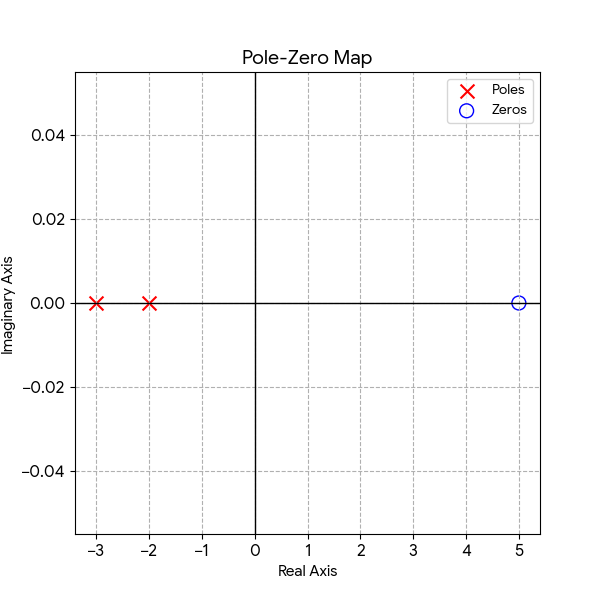
\includegraphics[width=0.6\columnwidth]{figures/Zeroes and Poles.png}
\caption{Poles and Zeroes}
\label{fig:placeholder}
\end{figure}
No poles in the Right Half Plane(RHP)
\end{frame}

\begin{frame}{Plot}
\begin{figure}[H]
\centering
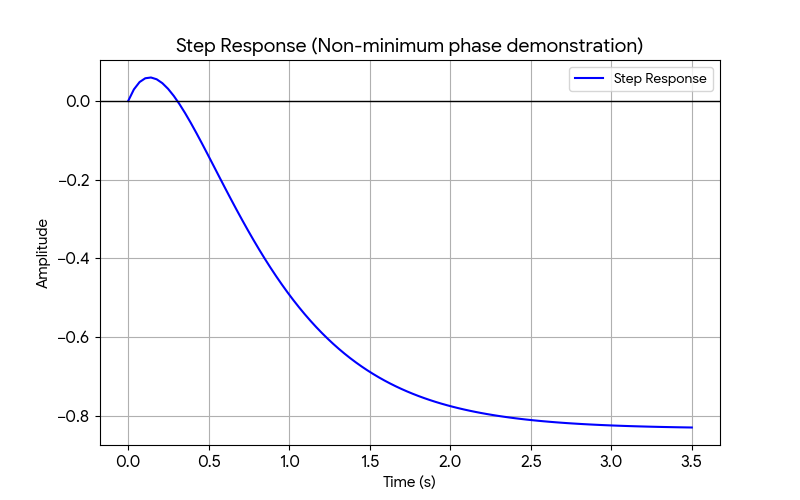
\includegraphics[width=0.6\columnwidth]{figures/Syablility.png}
\caption{Stability}
\label{fig:placeholder}
\end{figure}
$\rightarrow$ When Step signal is given as input, we can notice that the blue line eventually levels off (around $-0.83$). This proves the system is stable.\\
$\rightarrow$ Instead of going down toward the final value, the graph initially dips in the opposite direction.This proves the Non-Minimum phase of the system.
\end{frame}

\begin{frame}{Plot}
\begin{figure}[H]
\centering
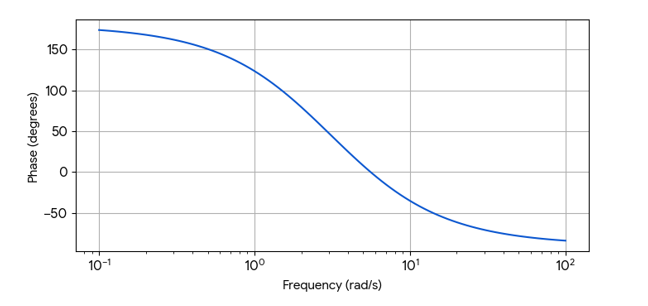
\includegraphics[width=0.75\columnwidth]{figures/Bode plot.png}
\caption{Bode Plots}
\label{fig:placeholder}
\end{figure}
\end{frame}

\begin{frame}
Phase: In a "Minimum Phase" system, the phase would drop a certain amount. But in this system, the RHP zero adds a massive amount of extra "Phase Lag."\\

Pole 1 (at -2): Contributes $-90^\circ$\\
Pole 2 (at -3): Contributes $-90^\circ$\\
Zero (at +5): Contributes $-90^\circ$ (Because it is in the RHP)\\
Total Phase Drop: $-90 + -90 + -90 = \mathbf{-270^\circ}$
\end{frame}
\begin{frame}{Unstable system Example}
    System:$$G_A(s) = \frac{1}{s - 1}$$
    Pole: $s = +1$\\
    Behavior: The output $y(t) \approx e^t$ grows exponentially.\\
\end{frame}

\begin{frame}[fragile]
\frametitle{Python code}
\begin{lstlisting}
import numpy as np
import matplotlib.pyplot as plt
from scipy import signal

t = np.linspace(0, 30, 1000)
sys_rhp = signal.TransferFunction([1], [1, -0.5])
t1, y1 = signal.step(sys_rhp, T=t)

# G(s) = 1 / (s^2 + 4) -> Poles at +/- 2j
sys_marginal = signal.TransferFunction([1], [1, 0, 4])
t2, y2 = signal.step(sys_marginal, T=t)
\end{lstlisting}
\end{frame}

\begin{frame}[fragile]
\begin{lstlisting}
# --- SYSTEM 3: Repeated Poles on Imaginary Axis ---
# G(s) = 1 / (s^2 + 4)^2 = 1 / (s^4 + 8s^2 + 16)
# Poles at +/- 2j (Repeated twice)
sys_repeated = signal.TransferFunction([1], [1, 0, 8, 0, 16])
t3, y3 = signal.step(sys_repeated, T=t)

# --- Plotting ---
plt.figure(figsize=(10, 10))
\end{lstlisting}
\end{frame}

\begin{frame}[fragile]
\begin{lstlisting}
# Plot 1: RHP Pole
plt.subplot(3, 1, 1)
plt.plot(t1, y1, 'r', label='Pole at s=+0.5')
plt.title('Unstable: Pole in Right Half Plane (Exponential Growth)')
plt.grid(True)
plt.legend()

plt.tight_layout()
plt.show()
\end{lstlisting}
\end{frame}

\begin{frame}{Plot}
\begin{figure}[H]
\centering
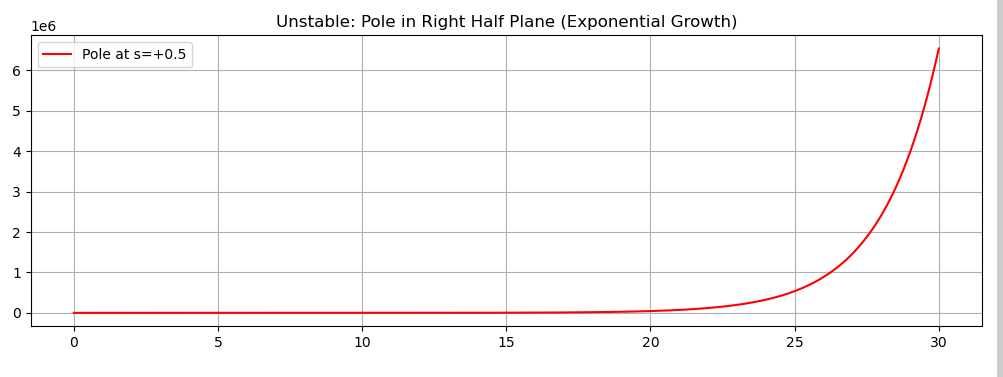
\includegraphics[width=0.65\columnwidth]{figures/Unstable.png}
\caption{Unstable system}
\label{fig:placeholder}
\end{figure}
 Even though the input is "small" (just 1: step input), the system cannot handle it. The internal energy builds up exponentially ($e^{at}$) because the pole is in the RHP. It will never settle.
\end{frame}

\begin{frame}{Uncontrollable system example}
    $$G(s) = \frac{s + 2}{(s + 2)(s + 3)}$$
    Poles: $s = -2, -3$\\
    Zeros: $s = -2$\\
    The $(s + 2)$ term appears in both the numerator and denominator. While a calculator might simplify this to $\frac{1}{s + 3}$, the physical state associated with the pole at $-2$ cannot be reached or controlled by the input.
\end{frame}

\begin{frame}[fragile]
\begin{lstlisting}
import numpy as np
import matplotlib.pyplot as plt
from scipy import signal

# Define the Uncontrollable System: G(s) = (s + 2) / [(s + 2)(s + 3)]
num = [1, 2]       # Represents (s + 2)
den = [1, 5, 6]    # Represents (s^2 + 5s + 6) which is (s+2)(s+3)

# Automatically find poles and zeros
zeros = np.roots(num)
poles = np.roots(den)
\end{lstlisting}
\end{frame}

\begin{frame}[fragile]
\begin{lstlisting}
# --- Plotting the Pole-Zero Map ---
plt.figure(figsize=(7, 6))

# Plot Poles as 'x'
plt.scatter(poles.real, poles.imag, marker='x', color='red', s=150, 
            label=f'Poles at {poles}')

# Plot Zeros as 'o'
plt.scatter(zeros.real, zeros.imag, marker='o', edgecolors='blue', 
            facecolors='none', s=100, linewidth=2, label=f'Zeros at {zeros}')
\end{lstlisting}
\end{frame}

\begin{frame}[fragile]
\begin{lstlisting}
# Add Axis lines and labels
plt.axvline(0, color='black', lw=1)
plt.axhline(0, color='black', lw=1)
plt.grid(True, linestyle='--', alpha=0.7)
plt.xlabel('Real Axis')
plt.ylabel('Imaginary Axis')

# Highlight the cancellation
plt.title('Pole-Zero Map: Uncontrollable System Demonstration')
plt.annotate('Cancellation! (Zero on top of Pole)', xy=(-2, 0), xytext=(-1.5, 0.5),
             arrowprops=dict(facecolor='black', shrink=0.05), fontsize=10)
\end{lstlisting}
\end{frame}

\begin{frame}[fragile]
\begin{lstlisting}
plt.legend()
plt.show()

# Print the numerical values for your instructor
print(f"Poles found at: {poles}")
print(f"Zeros found at: {zeros}")
print("Conclusion: Because a Zero cancels a Pole at s = -2, the system is Uncontrollable.")
\end{lstlisting}
\end{frame}

\begin{frame}{Plot}
\begin{figure}[H]
\centering
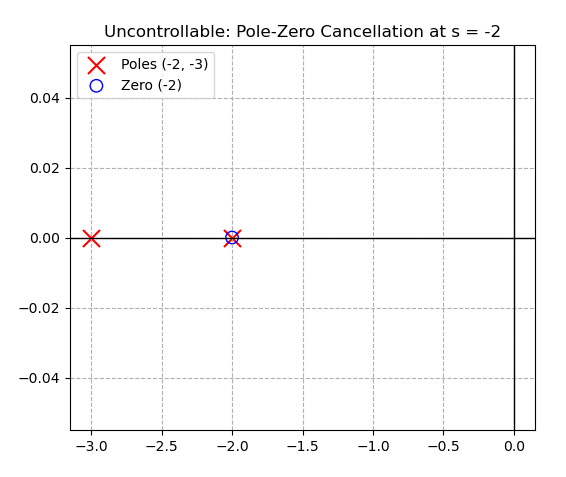
\includegraphics[width=0.65\columnwidth]{figures/Uncontrollable.png}
\caption{Uncontrollable system}
\label{fig:placeholder}
\end{figure}
\end{frame}

\end{document}